\documentclass{article}

% PACKAGES --------------------------------------
\usepackage[utf8]{inputenc}
\usepackage[T1]{fontenc}

% GENERAL --------------------------------------

\usepackage{tikz} % Drawings
\usepackage{wrapfig} % Inline images
\usepackage{amsmath,amssymb,amsthm} % Advanced math
\usepackage{xcolor} % Colored text
\usepackage{hyperref} % Clickable TOC
\renewcommand{\baselinestretch}{1.2} % Line height
\usepackage{graphicx} % Graphics *but better*

\graphicspath{{./img/}}

% SETUP ----------------------------------------------

\usepackage[toc]{glossaries}
\makeglossaries

% ACRONYM DEFINITIONS ----------------------------------------------

% Usage:
% \newacronym{label}{short}{long}

% GLOSSARY ENTRIES  ----------------------------------------------

% Usage:
% \newglossaryentry{label}
% {
%     name = name,
%     description = {my desc},
%     plural = {plural}
% }

\newglossaryentry{Algebra}
{
    name = Algebra,
    description = {Themengebiet der Mathematik, welches die Eigenschaften von Rechenoperation umfasst und mit Unbekannten in Gleichungen arbeitet}
}

\newglossaryentry{analytische Geometrie}
{
    name = analytische Geometrie,
    description = {Themengebiet der Mathematik, welches die Geometrie innerhalb eines Koordinatensystems umfasst}
}

\newglossaryentry{Analysis}
{
    name = Analysis,
    description = {Themengebiet der Mathematik, welches die Untersuchung von Funktionen beschreibt und die Methoden der \Gls{Differentialrechnung} und \Gls{Integralrechnung}, basierend auf der \Gls{Infinitesimalrechnung}}
}

\newglossaryentry{Binomialkoeffizient}
{
    name = Binomialkoeffizient,
    description = {Anzahl der $k$-elementigen Teilmengen einer $n$-elementigen Menge, geschrieben als $\binom{n}{k}$ sprich \say{$n$ über $k$}},
    plural = {Binomialkoeffizienten}
}

\newglossaryentry{Brechung}
{
    name = Brechung,
    description = {Auch Refraktion genannt, beschreibt die Veränderung der Richtung des Lichts bei einem Übergang in ein anderes Medium, in welchem es sich mit anderer Geschwindigkeit bewegt},
    plural = {Brechungen}
}

\newglossaryentry{Differentialrechnung}
{
    name = Differentialrechnung,
    description = {Teil des mathematischen Themengebiets Analysis, welches sich mit der Berechnung lokaler Veränderungen von Funktionen beschäftigt (Ableitung, Minima, Maxima etc.), basierend auf der \Gls{Infinitesimalrechnung}}
}

\newglossaryentry{Faktor}
{
    name = Faktor,
    description = {Bestandteile einer Multiplikation},
    plural = Faktoren
}

\newglossaryentry{Integralrechnung}
{
    name = Integralrechnung,
    description = {Teil des mathematischen Themengebiets Analysis, welches sich mit der Berechnung von Volumen oder Flächen von Funktionen beschäftigt, basierend auf der \Gls{Infinitesimalrechnung}}
}

\newglossaryentry{Infinitesimalrechnung}
{
    name = Infinitesimalrechnung,
    description = {Methode, um eine Funktion auf unendlich kleinen (infinitesimalen) Schritten zu beschreiben, Grundbaustein der \Gls{Differentialrechnung} und \Gls{Integralrechnung}}
}

\newglossaryentry{kartesisches Koordinatensystem}
{
    name = Kartesisches Koordinatensystem,
    description = {Ein orthogonales Koordinatensystem, dessen Koordinatenlinien Geraden in konstantem Abstand sind, verständlich als das grundlegende Koordinatensystem mit x- und y-Achse}
}

\newglossaryentry{Kongruenz}
{
    name = Kongruenz,
    description = {Die Beziehung zwischen zwei Zahlen, dessen \Gls{Modulo} mit demselben Divisors identisch ist},
    symbol = {\ensuremath{\equiv}},
    plural = {Kongruenzen}
}

\newglossaryentry{Modulo}
{
    name = Modulo,
    description = {Der Rest einer Division zweier Zahlen}
}

\newglossaryentry{Natuerliche Zahl}
{
    name = Natürliche Zahl,
    description = {Alle Zahlen, mit deren Hilfe beliebige Objekte gezählt werden können ($\mathbb{N} = \{ 1,2,3,4, \dots \}$)},
    plural = {Natürliche Zahlen}
}

\newglossaryentry{Optik}
{
    name = Optik,
    description = {Themengebiet der Physik, welches die Lehre des Lichts darstellt}
}

\newglossaryentry{Pascalsches Dreieck}
{
    name = Pascalsches Dreieck,
    description = {Form der grafischen Darstellung der Binomialkoeffizienten in einem Dreieck, bei dem jeder Eintrag die Summe der zwei darüberstehenden Einträge ist}
}

\newglossaryentry{Primzahl}
{
    name = Primzahl,
    description = {Eine natürliche Zahl, die ausschließlich durch 1 und sich selbst geteilt werden kann},
    plural = {Primzahlen}
}

\newglossaryentry{Quadratzahl}
{
    name = Quadratzahl,
    description = {Eine Zahl, die durch die Multiplikation einer ganzen Zahl mit sich selbst entsteht},
    plural = {Quadratzahlen}
}

\newglossaryentry{Stochastik}
{
    name = Stochastik,
    description = {Themengebiet der Mathematik, welches die Wahrscheinlichkeitsrechnung, sowie die Mathematische Statistik zusammenfasst}
}

\newglossaryentry{Unendlicher Abstieg}
{
    name = Methode des unendlichen Abstiegs,
    description = {Eine von Fermat entwickelte Methode, welche einen Beweis durch Widerspruch beschreibt, bei dem ein kleinstes Element in einer Zahlenmenge vorhanden sein muss, dem aber nicht so ist, oder umgekehrt, dass es kein kleinstes Element geben soll, aber eines existiert. Ähnlich zu einem Beweis durch Induktion}
}

\newglossaryentry{Zahlentheorie}
{
    name = Zahlentheorie,
    description = {Themengebiet der Mathematik, welches sich mit Eigenschaften ganzer Zahlen beschäftigt}
}
 % Glossary
% SETUP ----------------------------------------------
    \usepackage[intoc, german]{nomencl}
    \makenomenclature

% ENTRIES --------------------------------------------

    \nomenclature{$c$}{Lichtgeschwindigkeit, ca. $3 \cdot 10^8 \frac{m}{s}$}
    
    \nomenclature{$\in$}{Element einer Menge, Beispiel \say{$n \in \{2,4,5\}$}, sprich \say{$n$ ist ein Element von $\{2,4,5\}$}}
    
    \nomenclature{$\equiv$}{Kongruenz, Beispiel \say{$a \equiv b \pmod{m}$}, sprich \say{$a$ und $b$ sind kongruent modulo $m$}, bei der Division durch $m$ besitzen $a$ und $b$ den gleichen Rest}
    
    \nomenclature{$\binom{n}{k}$}{Binomialkoeffizient, sprich \say{$n$ über $k$}}
    
    \nomenclature{$a \mid b$}{Ganzzahlige Teilbarkeit, sprich \say{$a$ ist durch $b$ teilbar}}
    \nomenclature{$a \nmid b$}{Verneinung von $a \mid b$}
    
    \nomenclature{$\sum$}{Summe, griechischer Buchstabe Sigma, Beispiel $\displaystyle \sum^{10}_{n=1} n^2$ quadriert alle Zahlen von 1 bis 10 und addiert diese ($1^2 + 2^2 + ... + 10^2 = 385$)} % Nomenclature/Symbolverzeichnis

% MACROS ----------------------------------------

% Displaystyle fractions
\newcommand\ddfrac[2]{\ensuremath{\frac{\displaystyle #1}{\displaystyle #2}}}

% TIKZ ------------------------------------
\usepackage{pgf,tikz,pgfplots}
\usepackage{mathrsfs}
\usetikzlibrary[patterns]
\pgfplotsset{compat=1.15}
\usetikzlibrary{arrows}
\newcommand{\degre}{\ensuremath{^\circ}}

% GERMAN --------------------------------------

\usepackage[ngerman]{babel} % german
\usepackage{csquotes}

% https://www.overleaf.com/learn/latex/Typesetting_quotations
% use \say{} to quote something
\usepackage[
    left = \glqq{},
    right = \grqq{},
    leftsub = \glq{},
    rightsub = \grq{}
]{dirtytalk} % Correct quotation marks

\newtheorem*{theorem}{Hypothese} % Rename
\addto\captionsngerman{%
    \renewcommand{\abstractname}{Vorwort}
}

% BIBLIOGRAPHY --------------------------------------

\usepackage[backend=biber,sorting=none]{biblatex}
\addbibresource{lib/bib.bib}

% OPTIONS --------------------------------------

% SETUP --------------------------------------

    \title{Pierre de Fermat}
    \author{******** Nguyen}
    \date{Januar 2020}

% TEMPORARY -------------------------------------

    % \includeonly{sections/mathematik}

% DOCUMENT --------------------------------------

\begin{document}

% TITLE PAGE  --------------------------------------

\maketitle

\vspace{1cm}

\begin{center}
    \begin{tabular}{r|l}
        Kurs         & Seminarkurs Mathematik, Berühmte Mathematiker \\
        Lehrer       & ******** Schmidt                              \\
        Abgabetermin & 2019-01-08                                    \\
    \end{tabular}
\end{center}

\vspace{2cm}

\begin{abstract}
    In dieser Seminararbeit wird der Schwerpunkt auf Fermats Biografie, und auf seinen mathematischen Erfolgen stehen. Ich habe Fermat ausgewählt, da mir der kleine und große Satz von Fermat (den ich auch später behandeln werde) schon zu Ohren gekommen war. Der Großteil seiner Arbeit lag in der Zahlentheorie, ein Gebiet welches ich selber gerne mag. Interessant an Fermat ist außerdem, dass er von Beruf her gar kein Mathematiker, sondern Jurist war und Mathematik nur als Nebenhobby gemacht hat. Der biografische Teil wird seine juristische Karriere, aber auch Fermats Charakter beschreiben. Der mathematische Teil wird relativ viele Themengebiete decken, insgesamt Kurvenanalyse, Optik, Stochastik und Zahlentheorie. Der größte Fokus wird hierbei auf der Zahlentheorie liegen. Wer sich noch nicht viel mit Mathematik beschäftigt hat wird hier auf unbekannte Begriffe und Symbole treffen, daher habe ich im Glossar und im Symbolverzeichnis die meisten hinterlegt und erklärt.
\end{abstract}

\newpage

% TABLE OF CONTENTS --------------------------------------

\tableofcontents
\newpage

% PROOF OF OWNERSHIP --------------------------------------

\textit{Hiermit versichere ich, die vorliegende Arbeit selbstständig und nur unter Zuhilfenahme der angegeben Quellen und Hilfsmittel angefertigt zu haben. Aus den angegebenen Materialien entnommene Inhalte und Zitate sind als solche kenntlich gemacht. Ich erkläre, dass ich zu diesem Thema nicht schon einmal eine solche Arbeit angefertigt habe.}

% CONTENT --------------------------------------

\section{Biografie} \label{sec:bio}
    In diesem Abschnitt wird das Leben von Pierre de Fermat beschrieben.
    
    \subsection{Eltern} \label{sec:eltern}
        Fermats Vater war Dominique Fermat, ein reicher Verkäufer und Hersteller. Dominique tat sein Bestes um die Familie in Reichtum aufblühen zu lassen, indem er Tauschhandel mit verschiedenen Ländern trieb. Dabei handelte er mit landwirtschaftlichen Erzeugnissen, wie z.B. Weizen, Wein, Vieh und anderen Tierprodukten. Sein Geschick und sein Ansehen haben ihn so reich werden lassen wie er geworden ist. Pierres Mutter war Claire De Long, die zweite Frau Dominiques, welche aus einer edlen Familie von Juristen kam. Durch Dominiques Ehe mit Claire De Long hatte sich die Familie außerdem die Möglichkeit bekommen einen Platz im hohen Strafgericht von Toulouse für die beiden Söhne, Pierre und Clement, zu ergattern. Sie starb als Pierre nur sieben Jahre alt war.
        
    \subsection{Kindheit} \label{sec:kindheit}

        \begin{wrapfigure}{r}{0.25\textwidth}
            \centering
            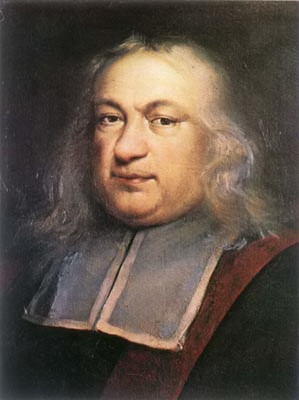
\includegraphics[width=0.25\textwidth]{img/Pierre_de_Fermat.jpg}
            \caption{Pierre de Fermat \cite{imgFermat}}
            \label{fig:fermat}
        \end{wrapfigure}

        Ein Rätsel von Pierre de Fermat fängt schon bei der Geburt an. In vielen Quellen wird beschrieben, dass sein Geburtsjahr 1601 sei. In diesem Gedanken hat man dann auch sein 400. Jubiläum im Jahr 2001 gefeiert. Sein Geburt hat sich aber schlussendlich als 1607 in Frankreich herausgestellt. \cite{whenWasFermatBorn} Grund für diese Verwechslung war wahrscheinlich sein verstorbener Halbbruder welcher auch Pierre Fermat hieß, der 1601 geboren war und dann noch in der Kindheit gestorben ist. \cite{famousScientistsFermat} Seine Karriere war von seinen Eltern bereits lange vorausgeplant, es ging ausschließlich darum sich einen Platz als parlamentarischen Berater in Toulouse oder Bordeaux zu erkaufen. Dafür muss man mehrere Jahre Jura studiert, einen Abschluss darin gemacht, dann noch mehrere Jahre als Anwalt entweder in Toulouse oder Bordeaux verbracht haben und zum Schluss eine Menge Geld aufbringen um den Platz zu erwerben. Er hat den Großteil seiner Kindheit an einer sprachen-zentrierten Schule verbracht, welche er im Alter von 16 Jahren abgeschlossen hatte. Dabei hat er wichtige Sprachen wie Griechisch, Latein, Italienisch und weitere gelernt und konnte diese auch flüssig sprechen, welche ihm in der späteren Laufzeit als Anwalt den Weg bahnen würde.

    \subsection{Studium} \label{sec:studium}
        Orléans war als \textit{die} Stadt bekannt, an der man am besten Zivilrecht studieren würde. Nicht nur in Frankreich, sondern in ganz Europa. Ein Abschluss von dort wurde als sehr hoch angesehen. Dort hat er dann auch an der Universität von Orléans im August 1626 seinen Abschluss gemacht als er nur 18 Jahre alt war. Darauf folgend hat sich Fermat im Strafgericht von Bordeaux einen Platz geschaffen. Er hat in Bordeaux die vier Jahre Praxiserfahrung als Anwalt, die für die Position des parlamentarischen Beraters notwendig sind, erhalten. Eigentlich war Toulouse eine ersichtlichere Wahl gewesen, aber er hatte sich für Bordeaux für den Mathematiker-Kreis entschieden, der sich dort gebildet hatte. Er hatte nämlich damals schon Interesse an der Mathematik gefunden und ist auf die Empfehlung seines Freundes nach Bordeaux gegangen.

    \subsection{Aufstieg zum parlamentarischen Berater} \label{sec:aufstieg}
        Als sein Vater Dominique Fermat im Juni 1628 gestorben ist, bekam Pierre den Großteil des Erbes und hat damit großen Reichtum erlangt, er bekam mit dem Erbe sechs Bauernhöfe, so wie mehrere andere Grundstücke. Danach hatte er auf eine Gelegenheit gewartet, um sich einen Platz als parlamentarischen Berater in Toulouse zu erkaufen, um dem Plan seiner Eltern nachzugehen. Diese Gelegenheit bot sich ihm, als 1630 ein Großteil der Berater einer Pest niedergefallen sind. Solch einen Platz zu erkaufen war keineswegs billig und nur mithilfe des Erbes seines Vaters möglich. Ein einfacher Bauer hatte damals 100 Livre im Jahr verdient, während man mit dem Platz als Berater leicht mehr als 45.000 Livre los wird.

        Im Jahr 1631 saß er dann endlich in seinem Büro als echter parlamentarischer Berater und durfte nun das \textit{\say{de}} in seinem Namen tragen und hieß damit offiziell \say{Pierre de Fermat} und nicht nur \say{Pierre Fermat}, wovon er persönlich aber nie wirklich Gebrauch gemacht hat. Um diese Zeit hat er auch seine Cousine, Louise de Long, geheiratet. Sie war zum Zeitpunkt der Hochzeit nur 15 Jahre alt. Insgesamt hatte er acht Kinder mit ihr, von denen nur fünf erwachsen geworden sind. 1637 stieg er zu einer höheren Position im Toulouser Strafgericht auf, diese Position hat er dann bis zu seinem Lebensende 1665 behalten. Mehr zu seiner Karriere als parlamentarischer Berater lässt sich in der Dezember 2001 Ausgabe der European Mathematical Society (EMS) finden. \cite{barnerNewspaper}
    
    \subsection{Mathematik} \label{sec:biografieMathematik}
        Wie für viele andere Mathematiker in der Zeit war die Mathematik für ihn nur eine Nebenbeschäftigung, da es den Beruf \say{Mathematiker} an sich noch nicht wirklich gab. Er hat zwar während seines Jura-Studiums in Orléans bereits Interesse an der Mathematik gefunden und sie auch aktiv verfolgt, aber weiterhin seinen Fokus auf das Anwaltsleben gelegt. Nach seinem Aufstieg als Berater hat er begonnen mit verschiedenen älteren Werken zu arbeiten, indem er sie restaurierte bzw. rekonstruierte. Oft hatte er mit anderen Mathematikern über einen Briefaustausch Kontakt, darunter René Descartes, Blaise Pascal und weitere.  Auch wenn er nur ein Hobbyist war und als Amateur bezeichnet wird, wird er als der größte Amateur-Mathematiker aller Zeiten angesehen. \cite{mlodinow2011wenn, britannicaFermat} Wie genau er zur Mathematik beigetragen hat, wird in Kapitel \ref{sec:mathematik} behandelt.
    
    \subsection{Als Person}\label{sec:person}
        Er hat viele wichtige Dinge entdeckt, aber hatte nicht das Verlangen diese zu veröffentlichen. Sein Sohn, Clement Samuel de Fermat, hatte nach Pierres Tod einige seiner Briefe und Randnotizen veröffentlicht. Seine Art findet sich auch in eben diesen Notizen wieder. 
        
        Im Briefaustausch mit anderen Mathematikern wurden sie oft von ihm aufgefordert ein bestimmtes Problem zu lösen, meist eins zu welchem er bereits eine Lösung hatte. Er bat sie also nicht einfach um Hilfe, sondern wollte nur schauen wie schnell sie das Problem lösen konnten. Oder er hat eine Aufgabe mit dem Resultat, aber ohne den Lösungsweg präsentiert, falls er denn doch mal etwas veröffentlicht hatte. Seinen Charakter könnte man gut als leicht arrogant bezeichnen. 
        
        Auch hat er immer behauptet eine bestimmte Behauptung bewiesen zu haben, schrieb aber nie den Beweis dafür auf. Darunter gehören zum Beispiel auch der Zwei-Quadrate-Satz und Fermats großer Satz, welche beide in Kapitel \ref{sec:zahlentheorie} behandelt werden. Am bekanntesten wird wohl für immer folgende Behauptung bleiben, welcher als Kommentar am Buchrand in seiner Kopie von \textit{\say{Arithmetica}} von Diophantus verfasst war. Dieser würde dann zu seiner berühmtesten Problemstellung werden, welche in Kapitel \ref{sec:grSatz} näher behandelt wird.

        \begin{quote}
            \say{\textit{Ich habe einen wahrlich wunderbaren Beweis für dieses Problem entdeckt, für den dieser Buchrand zu eng ist.}}\footnote{Cuius rei demonstrationem mirabilem sane detexi. Hanc marginis exiguitas non caperet.}
        \end{quote}

\section{Beiträge zur Mathematik} \label{sec:mathematik}
In diesem Abschnitt werden ein paar von Pierre de Fermats wichtigsten Beiträge zur Mathematik vorgestellt. Er war in vielen Teilgebieten der Mathematik aktiv. Erklärungen vieler Fachbegriffe und Symbole werden im Glossar auf Seite \pageref{sec:glossary} und im Symbolverzeichnis auf Seite \pageref{sec:symb} zu finden sein.

\subsection{Kurvenanalyse} \label{sec:kurvenanalyse}
1629 schon, als er nur 19 Jahre alt war und noch in Orléans studiert hatte, hatte er Interesse an der Mathematik gewonnen. Er begann verschiedene alte Bücher diesbezüglich zu lesen und auch zu rekonstruieren. Pierre de Fermat und René Descartes haben unabhängig voneinander, aber nahezu zeitgleich, die Grundbausteine für die \gls{analytische Geometrie} gelegt. Die analytische Geometrie beschreibt das Lösen geometrischer Probleme mit einem kartesischem Koordinatensystem, welches allgemein ein für uns heute noch einfaches Koordinatensystem mit x- und y-Achse beschreibt. Das Konzept eines kartesischen Koordinatensystems, welches von Descartes entwickelt wurde (und auch nach ihm benannt ist) war revolutionär und daher grundlegend für die analytische Geometrie. Fermats Idee war es, verschiedene geometrische Formen bestimmten \glslink{Algebra}{algebraischen} Formeln zuzuweisen, welche das zweite bahnbrechende Konzept der analytischen Geometrie bilden.

Im Alter von 21 machte er mit seinem Werk \textit{\say{Methodus ad disquirendam maximam et minimam et de tangentibus linearum curvarum}}\footnote{Methoden zur Bestimmung von Minima und Maxima und Tangenten an Kurven} seinen ersten, aber auch einer der wichtigsten, Beiträge zur \glslink{analytische Geometrie}{analytischen Geometrie} sowie zur \Gls{Differentialrechnung}. Ein aus dem Lateinischen ins Englische übersetzter Artikel ist in \cite{fermatMinMax} zu finden. Die Ergebnisse dieser hatte Fermat bisher nur im Briefaustausch mit anderen Mathematikern geteilt, erst 1636 ist es in Form eines Manuskripts veröffentlicht worden. Dabei hat er ein Verfahren entwickelt, mit welchem sich Maxima, Minima und Tangenten zu verschiedenen Arten von Kurven finden lassen, welches gleich zur heutigen Differentialrechnung ist. Aus seinen Ergebnissen ist er einen Schritt weiter gegangen und hat als Erstes die Fläche einer Funktion von verschiedenen Potenzfunktionen gefunden, welches der Grundansatz der \Gls{Integralrechnung} war. Die daraus folgende Formel wurde von Newton und Leibniz verwendet, um unabhängig voneinander den Fundamentalsatz der \Gls{Analysis} zu erstellen, welcher die Konzepte der Ableitung und der Integration miteinander verbindet.
\subsection{Optik} \label{sec:optik}
Fermat war mit dem Gesetz der \Gls{Brechung} in der \Gls{Optik}, welches Descartes in 1637 in seinem Werk vorgestellt hatte, unzufrieden. Dies, zusammen mit dem gleichzeitigen Erscheinen der beiden Werke über die \gls{analytische Geometrie}, entfachte eine Rivalerie zwischen den Beiden. 20 Jahre später hat Fermat das Problem neu behandelt und ist zu dem Schluss gekommen, dass Licht nicht den \textit{kürzesten} Weg, sondern den Weg der kürzesten Zeit nimmt. Dies wird auch das \say{Fermatsche Prinzip} genannt. Daraus ließ sich das Brechungsgesetz bilden, welches wir heute kennen. Dabei ist das Verhältnis der Sinusse der Eintritts- und Austrittswinkel gleich dem Verhältnis der Geschwindigkeiten, indem sich das Licht in beiden Medien bewegt, also $\frac{\sin\alpha}{\sin\beta} = \frac{c_1}{c_2}$. Das Beispiel einer Brechung hat man schon als Kind betrachten können, bei dem ein Strohhalm der ins Wasser ragt einen anderen Eintrittswinkel als Austrittswinkel besitzt. Wenn die Lichtgeschwindigkeit in einem Vakuum nun ca. $c_1 = 3 \cdot 10^8$ beträgt, aber die Lichtgeschwindigkeit im zu übergehenden Medium $c_2 = 2 \cdot 10^8$ beträgt, dann beträgt das Verhältnis von $\frac{c_1}{c_2} = \frac{3}{2}$. Da das Verhältnis der Sinusse gleich dem Verhältnis der Geschwindigkeiten sein muss, wäre beim Eintrittswinkel $\alpha = 30\degre$ der Austrittswinkel $\beta = 19.47\degre$, da $\beta = \arcsin(\sin(20\degre) / \frac{3}{2}) = 19.47\degre$, wie in Abbildung \ref{fig:brechung} zu sehen.

% Exported from the geogebra file

\begin{figure}[htbp]
    \centering
    \definecolor{cuevff}{rgb}{0.7686274509803922,0.8980392156862745,1}
    \definecolor{wrwrwr}{rgb}{0.3803921568627451,0.3803921568627451,0.3803921568627451}
    \definecolor{dbwrru}{rgb}{0.8588235294117647,0.3803921568627451,0.0784313725490196}
    \definecolor{rvwvcq}{rgb}{0.08235294117647059,0.396078431372549,0.7529411764705882}
    \definecolor{cqcqcq}{rgb}{0.7529411764705882,0.7529411764705882,0.7529411764705882}
    \begin{tikzpicture}[line cap=round,line join=round,>=triangle 45,x=1cm,y=1cm]
        \draw [color=cqcqcq,, xstep=1cm,ystep=1cm] (-3,-3) grid (3,3);
        \clip(-3,-3) rectangle (3,3);
        \draw [shift={(0,0)},line width=2pt,fill=black,fill opacity=0.10000000149011612] (0,0) -- (90:1.0218734981003337) arc (90:120:1.0218734981003337) -- cycle;
        \draw [shift={(0,0)},line width=2pt,fill=black,fill opacity=0.10000000149011612] (0,0) -- (-90:1.0218734981003337) arc (-90:-70:1.0218734981003337) -- cycle;
        \fill[line width=0pt,color=rvwvcq,fill=rvwvcq,fill opacity=0.2] (-2,0) -- (2,0) -- (2,-2) -- (-2,-2) -- cycle;
        \fill[line width=0pt,color=cuevff,fill=cuevff,pattern=north east lines,pattern color=cuevff] (-2,0) -- (-2,2) -- (2,2) -- (2,0) -- cycle;
        \draw [line width=2pt,color=dbwrru] (-1,1.7320508075688774)-- (0,0);
        \draw [line width=2pt,color=dbwrru] (0,0)-- (0.6840402866513374,-1.8793852415718169);
        \draw [line width=1.6pt,dash pattern=on 1pt off 1pt,color=wrwrwr] (0,-5.435849295235544) -- (0,3.59751242797139);
        \draw [line width=2pt] (-2,0)-- (2,0);
        \begin{scriptsize}
            \draw [fill=rvwvcq] (0,0) circle (2.5pt);
            \draw[color=rvwvcq] (0.15,0.22022051674979287) node {$M$};
            \draw [fill=rvwvcq] (-1,1.7320508075688774) circle (2.5pt);
            \draw[color=rvwvcq] (-0.9157689967624881,1.9471867285393538) node {$A$};
            \draw[color=black] (1,0.6187511810089223) node {$\alpha = 30.00\textrm{\degre}$};
            \draw [fill=rvwvcq] (0.6840402866513374,-1.8793852415718169) circle (2.5pt);
            \draw[color=rvwvcq] (0.811197215027076,-1.6600267197548177) node {$B$};
            \draw[color=black] (1,-0.3418099072053897) node {$\beta = 19.47\textrm{\degre}$};
            \draw[color=dbwrru] (-0.609206947332388,0.802688410666982) node {$h$};
            \draw[color=dbwrru] (0.5455101055209891,-0.8527466562555556) node {$h'$};
            \draw[color=wrwrwr] (0.11632323631884896,3.5515281205568745) node {$s$};
            \draw[color=black] (0.03457335647082225,-0.0454665927562934) node {$l$};
        \end{scriptsize}
    \end{tikzpicture}
    \caption{Beispiel einer Brechung}
    \label{fig:brechung}
\end{figure} % tikz

\subsection{Stochastik} \label{sec:stochastik}
Blaise Pascal, ein weiterer wichtiger Mathematiker aus dieser Zeit, war ein Brieffreund von Fermat. Gemeinsam haben sie in 1654 den Grundstein für die heutige \Gls{Stochastik} gelegt. Pascal hatte Fermat zwei Problemstellungen anvertraut, die sich mit dem damaligen Glücksspiel befassten. Man muss bedenken, dass es damals noch kein Konzept von Stochastik gab wie es heute existiert. Damals konnte man nur grob abschätzen, dass bei einem sechs-seitigen Würfel die Chance auf eine Sechs eben $\frac{1}{6}$ beträgt. Dass die Chance auf einen Sechser-Pasch $\frac{1}{6} \cdot \frac{1}{6} = \frac{1}{36}$ beträgt ist für uns heutzutage selbstverständlich, war damals aber eine revolutionäre Entdeckung. Eine Übersetzung des Briefaustausches zwischen Fermat und Pascal in 1654 findet sich in \cite{fermatPascalProb}.

\subsubsection{Würfelproblem}
Chevalier de Méré hatte Pascal gefragt, ob es profitabel wäre, auf einen Sechser-Pasch in 24 Würfen zu wetten. Nach den damaligen Faustregeln wäre es nämlich profitabel gewesen, rein mathematisch gesehen aber nicht. Wie erwähnt ist die Chance auf einen Sechser-Pasch $\frac{1}{6} \cdot \frac{1}{6} = \frac{1}{36}$, die Chance \textit{keinen} Sechser-Pasch zu würfeln daher $1 - \frac{1}{36} = \frac{35}{36}$. Die Chance 24-mal hintereinander keinen Sechser-Pasch zu bekommen ist $(\frac{35}{36})^{24} = 0.5086$, also etwas mehr als die Hälfte. Da die Chance auf einen Sechser-Pasch in 24 Würfen demnach $1-(\frac{35}{36})^{24}=0.4914$ ist, also unter $\frac{1}{2}$ liegt, ist das Spiel also nicht profitabel. Das Konzept der Multiplikation, Potenzierung und Addition von Wahrscheinlichkeiten ist im Briefaustausch zwischen Pascal und Fermat entstanden.

\subsubsection{Teilungsproblem}
Das bekanntere (und auch interessantere) der beiden Probleme ist folgender:

\begin{quote}
    Zwei Spieler spielen ein Glücksspiel gegeneinander, bei dem jeder Spieler in jeder Runde die gleiche Chance zu gewinnen hat und welches auf mehrere Runden gespielt wird. Beide legen einen Wetteinsatz fest, sodass sich im Pot dann der insgesamt zweifache Wetteinsatz befindet. Es wird solange gespielt, bis einer der Spieler $n$-mal gewonnen hat, der Gewinner bekommt den gesamten Pot, während der Verlierer nichts bekommt (Alles oder nichts). Was aber nun, wenn das Spiel aufgrund eines Außeneinflusses beim Spielstand $a:b$ abgebrochen werden muss? Wie verteilt man dann am gerechtesten den Pot?
\end{quote}

Zum einen könnte man vorschlagen, dass der Pot $1:1$ wieder an die Spieler zurückgegeben wird. Dann könnte aber der Spieler in Führung argumentieren, dass dieser den gesamten Pot bekommen solle, da er doch in Führung lag und sicher gewonnen hätte. Beide Lösungen sind nicht falsch, aber auch beide nicht richtig. Die Lösung, die Fermat und Pascal vorgeschlagen haben, berechnet die Gewinnwahrscheinlichkeiten der jeweiligen Spieler und teilt den Pot im Verhältnis der Wahrscheinlichkeiten auf. Fermat ist auf den Gedanken gekommen, dass es irrelevant sei, wie viele Runden man schon gewonnen hatte, sondern es einzig und allein relevant sei, wie viele Runden man zum Sieg noch braucht. Wenn ein Spieler nun noch $r=n-a$ Runden gewinnen muss und der andere Spieler $s=n-b$ Runden, dann ist das Spiel nach maximal $r+s-1$ Runden vorbei. Beim Spielstand $3:2$ bis zu $5$ Punkten braucht es also maximal $2+3-1=4$ Runden. Da jeder Spieler die gleiche Chance zu gewinnen hat, gibt es $2^{r+s-1}$ Möglichkeiten, wie sich das Spiel entwickeln könnte. Fermat konnte also alle Möglichkeiten tabellarisch notieren, zählen bei welchen welcher Spieler gewinnen würde und damit die Proportionen der Gewinnchancen nutzen um den Pot zu verteilen.

Pascal hatte den Ansatz noch verbessert, da je größer $r+s-1$, desto exponentiell schwerer wird es die gesamte Tabelle zu schreiben. Mit dem \glslink{Pascalsches Dreieck}{pascalschen Dreieck}, welches er damals entwickelt hatte, sowie einer Summenformel, ist er auf folgende Formel gekommen, wobei $\binom{r+s-1}{k}$ den \Glspl{Binomialkoeffizient} darstellt:

\[ \sum^{r-1}_{k=0} \binom{r+s-1}{k} : \sum^{s-1}_{k=0} \binom{r+s-1}{k} \]

Beim Beispiel von $3:2$ bis $5$ Punkten wäre das also ein Verhältnis von $11:5$ bzw. $0.6875:0.3125$.
\subsection{Zahlentheorie} \label{sec:zahlentheorie}
Auch wenn Fermat wichtige Beiträge zur Analysis und zur Stochastik geleistet hat, finden sich seine größten und bekanntesten Werke im Gebiet der \Gls{Zahlentheorie}. Dies war Fermats Lieblingsgebiet. Dabei spielt das Buch \textit{\say{Arithmetica}} von Diophantus eine wichtige Rolle, da es viele Ideen von Fermat im Gebiet der \Gls{Zahlentheorie} entfacht hat. Oft hat er Notizen oder neue Ideen an den Rand seiner Kopie von Arithmetica geschrieben. Die Bekanntesten seiner Ideen werden folgend vorgestellt. Wenn nicht anders beschrieben, dann sind alle Variablen grundsätzlich eine ganze Zahl ($\mathbb{Z}$).

Um die Kapitel \ref{sec:2sqr} und \ref{sec:faktorMethode} besser zu verstehen, muss das Konzept der \Gls{Kongruenz} in der \Gls{Zahlentheorie} erklärt werden.\footnote{Die Definition aller komplexen mathematischen Begriffe und Symbole sind, wie bereits erwähnt, im Glossar auf Seite \pageref{sec:glossary} und im Symbolverzeichnis auf Seite \pageref{sec:symb} zu finden.} Für die \Gls{Kongruenz} wird das Symbol \glssymbol{Kongruenz} verwendet. Grundlegend wird die Schreibweise \say{$a \equiv b \pmod{m}$} benutzt (sprich \say{$a$ und $b$ \glslink{Kongruenz}{kongruent} modulo $m$}), welche beschreibt, dass der Rest von $\frac{a}{m}$ und $\frac{b}{m}$ gleich ist. Als Beispiel kann lässt sich \say{$9 \equiv 17 \pmod{8}$} nehmen, da $9 : 8 = 1 \text{ Rest } 1$ und $17 : 8 = 2 \text{ Rest } 1$. Im Endeffekt ist es aber nichts anderes als $(a \bmod m) = (b \bmod m)$.

\subsubsection{Zwei-Quadrate-Satz} \label{sec:2sqr}
Fermat hat folgendes behauptet:

\begin{quote}
    Eine ungerade \Gls{Primzahl} kann als eine Summe von zwei \glslink{Quadratzahl}{Quadraten} $p = x^2 + y^2$ dargestellt werden, wobei $x$ und $y$ \glslink{Natuerliche Zahl}{natürlich} sind, wenn, und nur wenn $p \equiv 1 \pmod{4}$.
\end{quote}

Zur Einfachheit halber lässt sich die Bedingung \say{$p \equiv 1 \pmod{4}$} auch als \say{Wenn $p$ als $4n+1$ darstellbar ist} umformulieren. Schauen wir uns ein paar Beispiele an.

\begin{itemize}
    \item 17 ist \glslink{Primzahl}{prim} und kann als $4 \cdot 4 + 1$ dargestellt werden, daher ist der Zwei-Quadrate-Satz anwendbar: $17 = 4^2 + 1^2 = 16 + 1$
    \item 29 ist \glslink{Primzahl}{prim} und ist $4 \cdot 7 + 1$: $\quad 29 = 5^2 + 2^2 = 25 + 4$
    \item 37 ist \glslink{Primzahl}{prim} und ist $4 \cdot 8 + 1$: $\quad 37 = 6^6 + 1^2 = 36 + 1$
    \item 7 ist \glslink{Primzahl}{prim}, kann aber nicht als $4n + 1$ dargestellt werden, daher ist 7 auch nicht als eine Summe von zwei \glslink{Quadratzahl}{Quadraten} darstellbar.
\end{itemize}

Fermat hatte behauptet, den Zwei-Quadrate-Satz mit der \glslink{Unendlicher Abstieg}{Methode des unendlichen Abstiegs} bewiesen zu haben. Eine Erklärung der Methode ist im Glossar zu finden. Er hat aber,wie man es von ihm gewohnt war, keinen Beweis niedergeschrieben. Der erste Beweis kam von Leonhard Euler 1747, nachdem er mehrere Jahre damit verbracht hatte einen Beweis zu finden. Dieser hatte ebenfalls den \glslink{Unendlicher Abstieg}{unendlichen Abstieg} genutzt.
Mittlerweile existieren verschiedene Beweise, die auf verschiedenen Konzepten basieren, darunter ein Beweis welcher gaußsche Zahlen nutzt \cite{woodbury}, oder auch ein Beweis in einem einzigen Satz. \cite{zagier}

\subsubsection{Faktorisierungsmethode} \label{sec:faktorMethode}

\begin{figure}[htb]
    \centering
    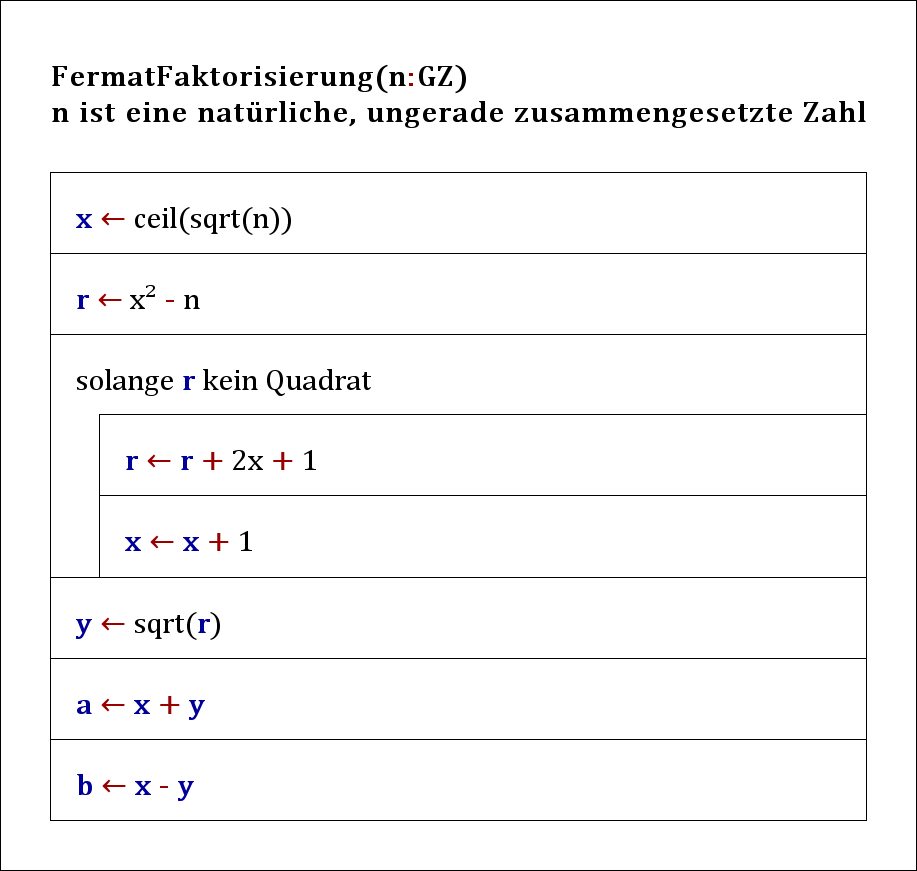
\includegraphics[width=0.75\textwidth]{img/factor_algorithm.png}
    \caption{Algorithmus von Fermats Faktorisierungsmethode in einem Struktogramm}
    \label{fig:factorAlgorithm}
\end{figure}

Die Faktorisierungsmethode von Fermat findet die \Glspl{Faktor} einer \glslink{Natuerliche Zahl}{natürlichen} ungeraden Zahl $n$, die aus mindestens zwei \Glspl{Primzahl} zusammengesetzt ist. Wenn die Faktorisierung von $n$ nun $n = a \cdot b$ ist, dann ist der Algorithmus für die Faktorisierungsmethode wie in Abbildung \ref{fig:factorAlgorithm} beschrieben. Dabei ist folgender Fakt grundlegend für die Faktorisierung:

\begin{theorem}
    Jede ungerade Zahl kann als eine Differenz von zwei \glslink{Quadratzahl}{Quadraten} dargestellt werden.
\end{theorem}
\begin{proof}
    Wenn man nun annimmt, dass sich eine ungerade Zahl $n$ auch als \begin{equation} \label{eq:faktor2square}
        n = x^2 - y^2
    \end{equation}
    schreiben lässt, ist es möglich mit der dritten binomischen Formel die Gleichung zu
    \begin{equation} \label{eq:binom}
        n = (x+y)(x-y)
    \end{equation}
    umzuschreiben. Nun setzt man eine Variable $a$ und $b$ gleich der beiden Faktoren aus \eqref{eq:binom}, sodass $a = x + y$ und $b = x - y$. Wenn man nun auf $x$ und $y$ auflöst, dann bekommt man $x = \frac{a+b}{2}$ und $y = \frac{a-b}{2}$. Eingesetzt in \eqref{eq:faktor2square} ergibt es

    \begin{align*}
        n & = \left( \frac{a+b}{2} \right)^2 - \left( \frac{a-b}{2} \right)^2 \\
          & = \dfrac{a^2 + 2ab + b^2 - a^2 + 2ab - b^2}{4}                    \\
          & = \dfrac{4ab}{4} = ab
    \end{align*}

    Somit kann jede ungerade Zahl kann als eine Differenz von zwei \glslink{Quadratzahl}{Quadraten} dargestellt werden.

\end{proof}

Dies wird nun genutzt, es wird solange eine Zahl $y$ gesucht, bis diese eine \Gls{Quadratzahl} ist. Da jede ungerade Zahl als Differenz von zwei \glslink{Quadratzahl}{Quadraten} dargestellt werden kann und eine dann bereits gefunden wurde, lässt sich die andere leicht durch Subtraktion finden. Nun hat man zwei Faktoren $a$ und $b$ von $n$ gefunden. Da $n$ ungerade ist, müssen die beiden Faktoren auch ungerade sein, da $n$ sonst gerade wäre. Wenn $a$ oder $b$ noch keine Primzahlen sind, dann kann man die gleiche Methode nutzen, um für jeweils $a$ oder $b$ die Faktoren zu finden. So hat Fermat bereits 1643 eine Primfaktorzerlegung von der Zahl $2.027.651.281$ durchgeführt. Auch dieser Beweis wurde von Fermat mit ins Grab genommen.

\subsubsection{Kleiner Satz} \label{sec:klSatz}
Fermats kleiner Satz ist der zweitbekannteste von Fermats Werken, nach dem großen Satz, er wird \say{klein} genannt, um ihn nicht mit dem Großen zu verwechseln. Dieser wurde 1640 in einem Brief von Fermat zu Bernard Frénicle de Bessy vorgestellt. Fermat hat den Satz als folgende Aussage vorgestellt:

\begin{quote}
    Wenn $p$ \glslink{Primzahl}{prim} und $a \nmid p$ ($a$ nicht durch $p$ teilbar), dann gilt
    \begin{equation} \label{eq:klSatz1}
        a^{p-1} \equiv 1 \pmod{p}
    \end{equation}
\end{quote}

\noindent Dies kann man auch als

\begin{quote}
    Wenn $p$ \glslink{Primzahl}{prim} und $a$ ganzzahlig, dann gilt
    \begin{equation} \label{eq:klSatz2}
        a^p \equiv a \pmod{p}
    \end{equation}
    sodass $a^p - a$ ein Mehrfaches von $p$ sein muss.
\end{quote}

\noindent formulieren, auch wenn die Anfangsbedingungen offener aussehen. Dies ist möglich, da die Formel \ref{eq:klSatz1} voraussetzt, dass $a \nmid p$. Daher muss es auch eine Zahl $b$ geben, sodass $ab \equiv 1 \pmod{p}$, da $a$ ansonsten keinen Teiler hätte. Wenn also nun $a^p \equiv a \pmod{p}$ und beide Seiten mit $b$ multipliziert werden, lässt sich auf beiden Seiten ein $a$ herauskürzen und es kommt $a^{p-1} \equiv 1 \pmod{p}$ heraus, welches somit äquivalent zu Formel \ref{eq:klSatz2} ist. Ein paar Beispiele:

\begin{itemize}
    \item Wenn $a=2$ und $p=5$, dann $2^{5} = 32 = 2 \cdot 16$. Damit lässt sich $2^{5}$ als ein Mehrfaches von 2 darstellen.
    \item Wenn $a=5$ und $p=13$, dann $5^{13} = 1220703125 = 5 \cdot 244140625$.
    \item $a=35$ und $p=19$: \quad $35^{19} = 217416671473944530487060546875 \\ = 35 \cdot 6211904899255558013916015625$
\end{itemize}

Mittlerweile gibt es einige Methoden um den Satz zu beweisen. Anders als der Beweis des großen Satzes von Fermat, passt der des kleinen Satzes leicht auf die Rückseite einer Postkarte. Da alle aber für den durchschnittlichen Leser etwas schwerer zu verstehen sind, werde ich darauf verzichten einen zu umfassen. Ein Beweis mit dem binomischen Lehrsatz lässt sich in \cite{wolframFlT} finden. Der Beweis von Fermat selber ist, wie man es sich schon denken kann, nirgendwo zu finden.

Auf dem kleinen Satz aufbauend ist der Satz von Euler, welcher eine Verallgemeinerung des kleinen Satzes darstellt, wobei $p$ nicht \glslink{Primzahl}{prim} sein muss. Der kleine Satz wird heutzutage als Basis für den fermatschen Primzahltest und in der heutigen Kryptografie als Basis der RSA-Verschlüsselung genutzt.

\subsubsection{Großer Satz} \label{sec:grSatz}
Der große Satz von Fermat, auch \say{Fermats letzter Satz} oder \say{Fermatsche Vermutung} genannt, ist sein bekanntestes Problem. Der Name \say{Fermats letzter Satz} kommt nicht daher, dass es wortwörtlich der letzte Satz war den er aufgestellt hatte, sondern weil es der Satz von Fermat war, der als letztes bewiesen wurde. Den großen Satz bzw. die Problemstellung, sowie den Beweis, hat er selbst nie veröffentlicht. Erst fünf Jahre nach seinem Tod hat einer seiner Söhne die zahlreichen Randnotizen in Fermats Kopie von Diophantus \say{Arithmetica} gefunden und veröffentlicht. Aufgestellt in ca. 1637 findet sich folgende Notiz am Rande:

\begin{quote}
    \textit{\say{Es ist unmöglich eine Zahl dritter Potenz in zwei Zahlen dritter Potenzen, oder eine Zahl vierter Potenz in zwei Zahlen vierter Potenzen, oder allgemein, jede Potenz höher als 2 in die zwei gleichen zu zerlegen. Ich habe einen wahrlich wunderbaren Beweis für dieses Problem entdeckt, für den dieser Buchrand zu eng ist.}}
    \footnote{Cubum autem in duos cubos, aut quadratoquadratum in duos quadratoquadratos \& generaliter nullam in infinitum ultra quadratum potestatem in duos eiusdem nominis fas est dividere cuius rei demonstrationem mirabilem sane detexi. Hanc marginis exiguitas non caperet.}
\end{quote}

Allgemein formuliert bedeutet das:
\begin{quote}
    Die Gleichung $x^n + y^n = z^n$ mit $n,x,y,z \in \mathbb{N}$ hat für $n>2$ keine ganzzahlige Lösung.
\end{quote}

Dass es für $n = 2$ unendlich viele Lösungen gibt, wussten schon die Griechen. Man muss nur das Stichwort \say{Satz des Pythagoras} sagen und es sollte einem direkt die Zahlengruppe $3,4,5$ einfallen, welche für $n = 2$ die gültige Lösung $3^2 + 4^2 = 5^2$ bildet. Zwar hat Fermat nicht den gesamten Satz bewiesen, dafür aber den Fall $n = 4$ mit seiner eigen entwickelten Methode des \glslink{Unendlicher Abstieg}{unendlichen Abstiegs}, dessen Beschreibung im Glossar zu finden ist.

Einfach zu verstehen wie er war, haben viele Mathematiker versucht den großen Satz von Fermat zu beweisen, jedoch sind alle am Versuch gescheitert. Über mehrere Jahrhunderte blieb die Lösung ein Mysterium. Erst 350 Jahre später hat Andrew Wiles 1995 einen kompletten Beweis des großen Satz von Fermat veröffentlicht. Dieser war schon seit seiner Kindheit, als er zehn Jahre alt war, von der Einfachheit des großen Satzes fasziniert und hat sich seitdem vorgenommen, diesen als Erstes zu beweisen. Da er aber schnell gemerkt hatte, dass es mit seinem mathematischen Wissen zu dieser Zeit nichts werden könne, hat er, erst nachdem er 33 geworden war, die Suche fortgesetzt. Nach mehr als 6 Jahren geheimgehaltener und akribischer Forschung hatte er 1993 den Beweis vorgetragen, mit dem Titel \say{Modular Forms, Elliptic Curves and Galois Representations.}. Dieser hatte sich nicht anmerken lassen, dass es sich hierbei um den Beweis Fermats großen Satz handelt. Erst am Ende des dritten und letzten Vortrags hat er nebenbei angemerkt, dass er nun den Satz bewiesen hatte. \cite{newYorkTimes} Im August wurde aber ein Fehler im Beweis entdeckt, den Wiles erst in September 1994 korrigieren konnte und Mai 1995 dann neu veröffentlicht hat. Für den Beweis hat er viele Preise und Auszeichnungen erhalten und er gilt als eines der wichtigsten Fortschritte der modernen Mathematik.

Den großen Satz hier zu beweisen würden den kompletten Rahmen der Arbeit sprengen. Wer einen Blick in Wiles 109 Seiten langen Beweis werfen möchte, findet diesen in \cite{wilesFermat}. Der Beweis behandelt den Modularitätssatz (früher auch \say{Taniyama-Shimura-Vermutung} genannt) und elliptische Kurven. Wiles beweist den schwierigsten Teil davon, welches gleichzeitig den großen Satz impliziert. Der vollständige Beweis des Modularitätssatzes ist 2001 gefunden worden. Ein Buch, welches den großen Satz und damit auch den Modularitätssatz weiter im Detail behandelt findet sich hier \cite{darmon}.

Der Beweis des großen Satzes wurde erst nach 6 Jahren Forschungen mit mathematischen Mitteln des 20. Jahrhunderts gefunden, daher ist man sich heutzutage einig, dass Fermat zwar behauptet hat einen Beweis gefunden zu haben, aber doch nie einen hatte oder dass sein Beweis fehlerhaft war.


\newpage

% OTHER --------------------------------------

\label{sec:glossary}
\printglossary
\label{sec:symb}
\printnomenclature
\newpage

\printbibliography[heading=bibintoc]

\end{document}
